\section{Фундаментальные взаимодействия и фундаментальные частицы (лептоны, кварки и переносчики
взаимодействий). Кварковая структура адронов.}

Элементарные частицы описываются \textit{стандартной моделью} и делятся на несколько основных классов:

\begin{itemize}
    \item \textit{Лептоны} -- электрон, мюон, таон, имеющие заряд $-1$ и спин $1 / 2$ и нейтральные лептоны (нейтрино), соответствующие им. Не участвуют в сильном взаимодействии.
    \item \textit{Кварки} -- элементарные частицы, из которых состоят все тяжёлые частицы, такие как нуклоны. Кварки имеют дробные электрические заряды $2 / 3$ или $- 1 / 3$. Кварки делятся на три поколения, в каждом из которых по два кварка с разными зарядами. С поколением растёт масса кварков.
    \item \textit{Бозоны} -- частицы, являющиеся переносчиками взаимодействия. Фотоны осуществляют электромагнитное взаимодействие, $Z$- и $W$-бозоны осуществляют слабое взаимодействие, глюоны осуществляют сильное взаимодействие между кварками (сильное взаимодействие между нуклонами переносится $\pi$-мезонами). 
\end{itemize}

\noindent
Лептоны и кварки являются фермионами.

\begin{figure}[htbp]
    \centering
    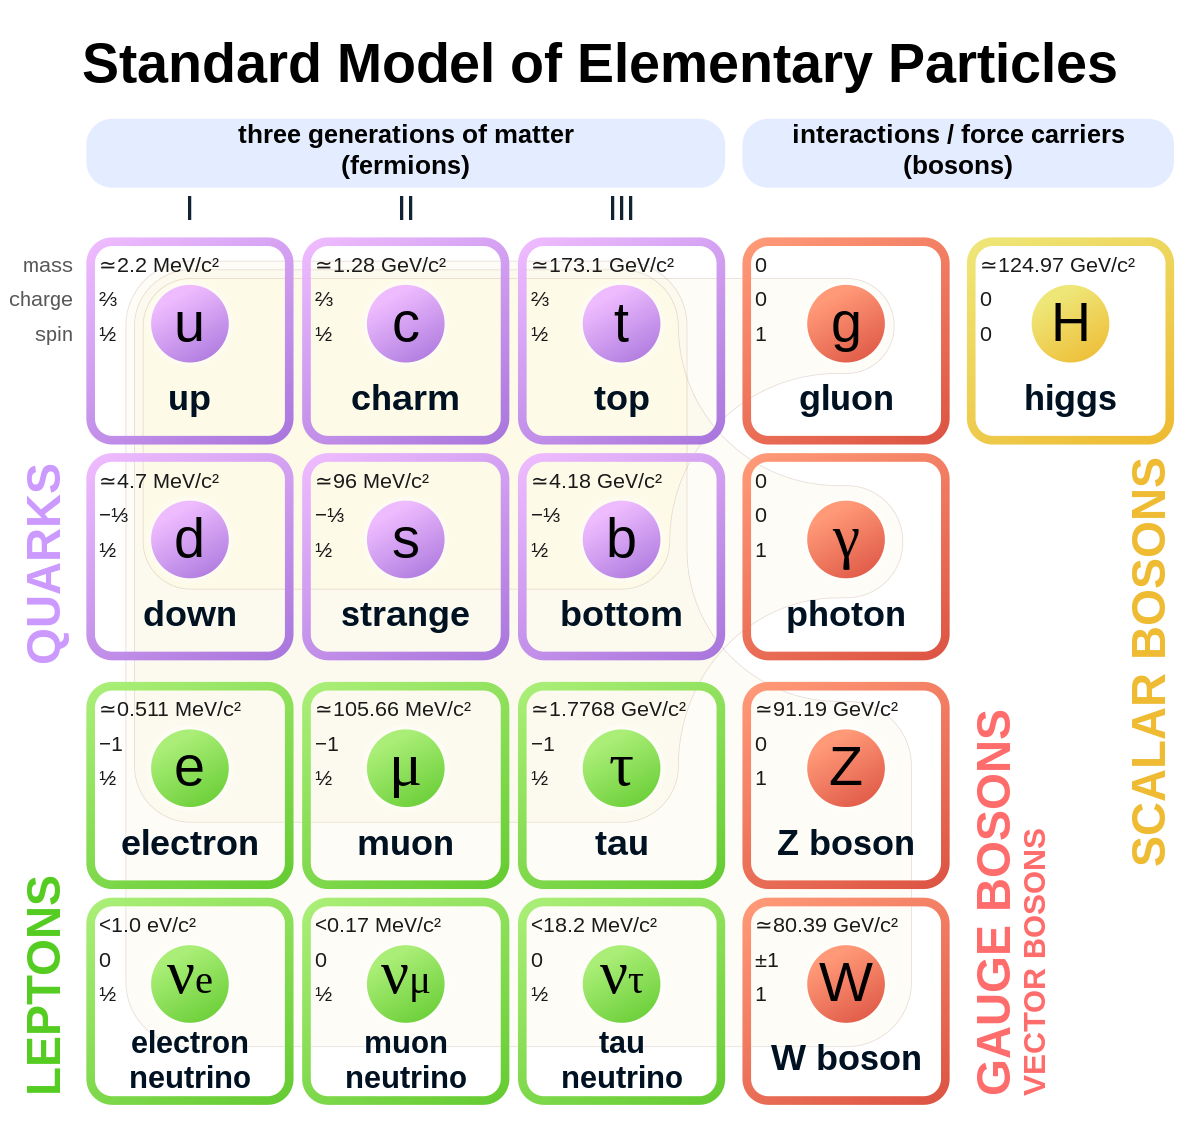
\includegraphics[width=0.5\linewidth]{63_стандартная_модель.png}
    \caption{Частицы стандартной модели}
    \label{fig:стандартная модель}
\end{figure}

\textit{Фундаментальные взаимодействия} -- различные типы взаимодействия между элементарными частицами. Это

\begin{itemize}
    \item \textit{Гравитационное} взаимодействие
    \item \textit{Электромагнитное} взаимодействие
    \item \textit{Сильное} взаимодействие
    \item \textit{Слабое} взаимодействие
\end{itemize}

Состоящие из кварков частицы называются \textit{адронами}. В основном наблюдаются \textit{мезоны} -- частицы, состоящие из двух кварков (кварк + антикварк), и \textit{барионы} -- частицы, состоящие из трёх кварков. Возможные и другие частицы (тетракварки, пентакварки), однако они существуют малое время.

\noindent
Обычных квантовых чисел оказывается недостаточно, чтобы описать кварки. Так, например, существуют частицы, состоящие из трёх кварков в одинаковом состоянии, что невозможно для ферми-частиц. Таким образом существует ещё одно квантовое число -- \textit{цвет} кварков. Адроны в целом \textit{бесцветны}, то есть либо присутствуют все возможные цвета (для барионов) либо цвет и антицвет (для мезонов). Глюонное взаимодействие кварков внутри частицы заключается в <<перекрашивании>> -- переносе цветового заряда между кварками.

Из-за глюонного взаимодействия оказывается невозможным существование свободных кварков. При, например, отдалении одного из кварков нейтрона от других, между ними образуется глюонная трубка, в которой накапливается энергия. При дальнейшем удалении энергии оказывается достаточно для образования новых частиц, что приводит к образованию двух адронов. С другой стороны, при больших энергиях столкновение частиц можно рассматривать как столкновение отдельных кварков друг с другом, поскольку энергия глюонной связи оказывается сравнительно мала.

$W$- и $Z$-бозоны могут осуществлять превращение одних кварков в другие (слабое взаимодействие).